\documentclass{article}
\usepackage[utf8]{inputenc}
\usepackage[left=3cm,top=3cm,right=3cm,bottom=3cm]{geometry}
\newcommand*\chem[1]{\ensuremath{\mathrm{#1}}}
\usepackage{amsmath}
\usepackage{mathtools}

\usepackage{natbib}
\usepackage{graphicx}
\usepackage{siunitx}

\let\oldthebibliography\thebibliography
\let\endoldthebibliography\endthebibliography
\renewenvironment{thebibliography}[1]{
  \begin{oldthebibliography}{#1}
    \setlength{\itemsep}{0em}
    \setlength{\parskip}{0em}
}
{
  \end{oldthebibliography}
}

\begin{document}

\begin{center}
\Huge
Identificación y exfoliación de monocristales de calcogenuros de metales de transición unidimensionales.

\vspace{3mm}
\Large Jesús David Rincón Puche

\large
201126021

\Large José Alejandro Montaña Cortés
\large 


\vspace{2mm}
\Large
Director: Paula Giraldo Gallo\\


\normalsize
\vspace{2mm}

\today
\end{center}

\begin{abstract}

En este proyecto se obtendrá una caracterización química, morfológica y estructural de monocristales de calcogenuros de metales de transición, particularmente los basados en Niobio y telurio ($Nb$ y $Te_2$), por medio de difracción de rayos X y Espectroscopía de energía dispersa. Seguido de esto, se realizará una exfoliación mecánica para reducir los monocristales a altura de capas atómicas y con microscopía de fuerza atómica (AFM) se caracterizarán las alturas de estas monocapas. Finalmente, se encontrará, usando espectroscopía Raman, la dependencia del corrimiento de los picos de Raman con el número de capas atómicas.

\end{abstract}

\normalsize
\section{Introducción}

Los calcogenuros de metales de transición son unos materiales muy fascinantes, dada la facilidad que tienen para cambiar sus propiedades físicas con ligeros cambios en su composición química. Estos son materiales interesantes para el estudio de propiedades tanto ópticas como eléctricas~\cite{dical}, dado que al cambiar su composición a través del dopaje se observan fenómenos físicos como superconductividad, Onda Densidad de Carga~\cite{CDW} (CDW, por sus siglas en inglés), entre muchos otros. En esta familia de materiales, se han encontrado algunos que presentan propiedades unidimensionales, y por lo mencionado anteriormente, es interesante desarrollar un estudio para entender de mejor manera las propiedades químicas asociadas a estos monocristales.\\

Por esta razón, el objetivo de este proyecto es realizar una caracterización química de estos materiales, particularmente los basados en $Nb$ y $Te$ usando difracción de rayos X; segundo, se encontrará la razón entre el $Nb$ y el $Te$ usando  Espectroscopía de energía dispersa (EDS, por sus siglas en inglés). Seguido de esto, se realizará una revisión bibliográfica sobre las propiedades físicas que estas combinaciones poseen. Una vez toda esta información esté conocida, se realizará una exfoliación para reducir la altura de los monocristales hasta capas atómicas, las cuales se caracterizarán con microscopía de fuerza atómica (AFM, por sus siglas en ingles) y por último realizar espectroscopia Raman para analizar la dependencia del corrimiento Raman de picos característicos con el número de capas atómicas.

\section{Estado del arte}
\subsection{Calcogenuros de metales de transición}

Algunos de los materiales que más atención han recibido recientemente son los calcogenuros de metales de transición. Estos materiales están constituidos por un metal de transición y un número de calcógenos (Por ejemplo, dos calcógenos generan un dicalcogenuro) y son materiales interesantes para el estudio en óptica en el área de fotónica y aplicaciones en optoelectrónicas al igual que estudios en nanoelectrónica~\cite{dical}. Además de esto, estos materiales son extremadamente sensibles a perturbaciones externas las cuales generan un gran cambio en sus propiedades físicas~\cite{dical}. En el área de la superconductividad, son materiales dónde se ve una competencia entre la superconductividad (SC) y la onda densidad de carga (CDW) donde se ha visto que al dopar dicalcogenuros, la fase SC se ha fortalecido mientras que la CDW se ha debilitado, dependiendo del dopaje~\cite{Competition1}. Lo último consiste en mantener el mismo número de portadores de carga al cambiar el calcógeno original y dopar con un metal diferente o reemplazar el metal por uno de igual valencia.\\

Las propiedades mencionadas están presentes en la mayoría de familia de estos materiales, particularmente aquellos que son capas de materiales unidimensionales con una estructura de cadena única y son muy útiles para aplicaciones en transistores de efecto campo, en fotodetectores de luz infrarroja, visible y ultravioleta y en la próxima generación en electrónica~\cite{trical}.\\

En adición, se han realizado estudios en vidrios de en cristales de calcogenuros, en este caso dicalcogenuros, de $As-Sb-S-I$ para encontrar su espectro Ramán al variar su composición para así encontrar como varían las propiedades mecánicas del bulk~\cite{PRABHUDESSAI201956}. Se observó que el corrimiento de los picos a niveles muy pequeños (capas atómicas) con cada cambio estructural, lo cual se relacionó con los cambios en las propiedades mecánicas~\cite{PRABHUDESSAI201956}.\\

En este proyecto, se realizará una caracterización del espectro de Raman para materiales unidimensionales en función del número de capas atómicas, al igual que se ha visto en dicalcogenuros de metales de transición.

\section{Objetivos}
\subsection{Objetivo general}

Determinar la dependencia de algunas propiedades físicas de monocristales unidimensionales de calcogenuros de metales de transición, particularmente los basados en $Nb$ y $Te$, como el espectro Raman en función del número de capas atómica mediante procesos de exfoliación mecánica.

\subsection{Objetivos Específicos}

\begin{enumerate}
    \item Realizar la caracterización química de monocristales de calcogenuros de metales de transición unidimensionales por medio rayos x y EDS (Energy dispersive Spectroscopy).
    \item Reducir las capas de estos materiales unidimensionales a sus alturas mínimas (idealmente un par de capas atómicas) por medio de procesos de exfoliación mecánica.
    \item Caracterizar con microscopia de fuerza atómica y espectroscopia Raman tanto para el bulk como para las muestras exfoliadas, para conocer la dependencia del corrimiento Raman de picos característicos con el número de capas atómicas.
\end{enumerate}

\section{Metodología}
La metodología a implementar para este proyecto consta de 3 partes principales:
\begin{enumerate}
    \item Realizar una caracterización de la fase química de monocristales por medio de:
    \begin{itemize}
        \item Rayos X
        \item EDS (Energy dispersive Spectroscopy)
    \end{itemize}
    \item Realizar una revisión bibliográfica de los materiales sintetizados con el fin de estudiar sus propiedades electrónicas.
    \item Efectuar una caracterización con:
    \begin{itemize}
        \item Microscopia de fuerza atómica.
        \item Espectroscopia de Raman
    \end{itemize}
    para las muestras completas como para las exfoliadas de forma mecánica.
\end{enumerate}
Con el fin de tener en cuenta las posibles fuentes de error se identifican los parámetros a tener en cuenta para cada medición anteriormente descrita.

\subsection{Difracción de rayos x}

Se usará la difracción de rayos X para la caracterización química del material. Esta técnica consiste en un haz de rayos X pasando a través de un conjunto de átomos, los cuales interactúan con dicha onda incidente generando dispersiones de tipo elástico e inelestástico~\cite{xrays}. Generalmente, la mayoría de los choques son de tipo inelástico, formando el diagrama de dispersión que permite conocer la distribución de los átomos dispersores. Por esta razón, este diagrama depende de la estructura de los átomos.\\

Entre sus características principales se encuentran: Poseer un longitud de onda parecida al espacio interplanar de los sólidos; una técnica no destructiva y no necesita una preparación específica para que las muestras sean analizadas~\cite{xrays}. 

Para este proyecto, se usará difracción de rayos X de polvo y difracción de rayos X de monocristal.

\subsection{Energy Dispersive Spectroscopy (EDS)}

La espectroscopia de energía dispersa (EDS), es una técnica de microanálisis químico que se usa en conjunto con microscopía de escaneo electrónico (SEM). Esto consiste en detectar los rayos x emitidos por una muestra cuando esta es  bombardeada por una rayo de electrones y de esa manera detectar la composición química de dicha muestra. Propiedades o fases del tamaño de \SI{1}{\micro\metre} o menos~\cite{EDS}.\\

Cuándo la mezcla es bombardeada por electrones, los electrones reflejados permiten obtener el espectro característico como se muestra en la figura \ref{EDS}\\ 

\begin{figure}
    \centering
    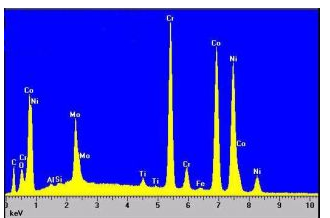
\includegraphics{Proyecto_final/Propuesta/EDSDiagram.png}
    \caption{Espectro de elememtos obtenido con EDS tomado de \cite{EDS}}
    \label{EDS}
\end{figure}

Junto a otras aplicaciones como lo son un mapeo de los elementos dentro de la muestra~\cite{EDS}.\\\

En cuanto a calibración, las muestras deben ser preparadas con diametros entre 200 $mm$ y 300 $mm$ y una altura de 50 $mm$ y soportar una presión de máximo 2 $Torr$.

Con esta técnica se hallará la razón entre el $Nb$ y el $Te$ presente en los monocristales de los calcogenuros.

\subsection{Microscopía de fuerza atómica}

La microscopia de fuerza atómica (AFM, por sus siglas en inglés) crea un perfil en 3D del material en escala nanoscópica, al medir las fuerzas entre una sonda aguda (10 nm) y la superficie (una distancia entre 2 y 10 nm)~\cite{AFM}. La sonda está sobre un cantiliver flexible, la cual podemos suponer como un resorte con su respectiva constante $k$, y mide la fuerza al tocar suavemente la superficie del material.

Por ende, el principio físico con el que se mide esto es la ley de Hook:

\[F=kx,\]

Normalmente $k$ tiene un valor entre 0.1 a 1 $N/m$~\cite{AFM}. Estas sondas normalmente están hechas de $Si_3N_4$ o $Si$. 

El montaje del AFM es el que se ve en la figura \ref{AFM}

\begin{figure}
    \centering
    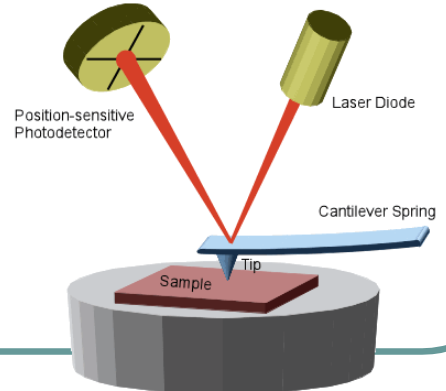
\includegraphics[scale=0.6]{Proyecto_final/Propuesta/AFM.png}
    \caption{Montaje AFM tomado de \cite{ClaseAFM}}
    \label{AFM}
\end{figure}

Como se observa, está compuesto por un foto detector, el cantiliver y un láser que golpea y va al detector. Luego toda esta información es registrada en un computador para mostrar los perfiles antes mencionados.

 Este microscopio más allá de las asombrosas y detalladas imágenes que puede obtener de las superficies de distintos materiales, proporciona una gran información de las fuerzas e interacciones que ocurren en un material de forma local. Sin embargo, la adquisición de estos datos depende fuertemente de un conocimiento previo de las propiedades físicas del ``resorte'' (cantilever) y la punta de la sonda. Es por esto que resulta ser clave lograr calibrar cada uno de estos elementos, el problema es que en la mayoría de los casos estos valores se toman de resultados teóricos o son supuestos del proveedor de fabrica. Esto tiene como consecuencia que se ignora la posibilidad de que haya variaciones en la fuerza debido a defectos estructurales\footnote{Esto puede deberse también debido a que los cantilevers son hechos con oro o con silicio o nitrógeno y silicio.} en la geometría o en la composición.
 
 Esta microscopía permite encontrar la altura de los cristales exfoliados mecánicamente.

\subsection{Espectroscopía Raman}
Dado que en la espectroscopía de Raman, un pico nace como respuesta a una estimulo de una cierta longitud de onda dada $\lambda_i$ cuando una muestra está siendo excitada con otro longitud de onda $\lambda_0$y, cuya forma funcional puede ser escrita como:
\[\nu_{i}=\frac{1}{\lambda_0}-\frac{1}{\lambda_1},\]
Esta excitación está asociada a una vibración molecular especifica.
 De lo anterior se observa entonces que la medición de $\lambda_0$ resulta relevante a la hora de lograr efectuar una buena calibración del espectrómetro.

Esta respuesta está asociada a una vibración molecular especifica $\omega$.

Como se menciona en el estado del arte, se ha visto una relación entre el corrimiento de los picos, y el número de capas atómicas (para dicalcogenuros), la cual se planea encontrar con esta técnica.


\section{Cronograma}

\begin{table}[htb]
	\begin{tabular}{|c|cccccccccc|}
	\hline
	Tarea $\backslash$ Semana & 1 & 2 & 3 & 4 & 5 & 6 & 7 & 8 & 9 & 10\\
	\hline
	1 & X & X &  &  &   &   &   &  &  &        \\
	2 &   & X & X&  &  &  &  &   &   &   \\
	3 &   &   &   & X  &   &   &   & &   &    \\
	4 & & & & X& X& & & & &               \\
	5 &  &  &  &  &  & X &  X& X & X &     \\
	6& & & & & & & & &X & X              \\
	\hline
	\end{tabular}
\end{table}
\vspace{1mm}

\begin{itemize}
	\item Tarea 1: Caracterización con difracción de rayos X y EDS
	\item Tarea 2: Búsqueda de bibliografía para propiedades físicas relacionadas con la caracterización.
	\item Tarea 3: Presentación con mitad de proyecto.
	\item Tarea 4: Familiarización con exfoliación mecánica.
	\item Tarea 5: Espectroscopia Raman y AFM.
	\item Tarea 6: Escritura informe final y preparación del póster final. 

\end{itemize}

\section*{Firma del Director}
\vspace{1.5cm}


\bibliographystyle{unsrt}
\bibliography{references}
\end{document}



